\begin{listing}[]
\centering
\begin{minipage}{.33\textwidth}
\begin{minted}
[
fontsize=\footnotesize,
linenos=true,
escapeinside=||,
breaklines
]
{go}
package main
import "sync"

type Container struct{ |\label{bugListing:containerType_start}|
  sync.Mutex
  stop  chan struct{}
} |\label{bugListing:containerType_end}|

func main() {
  container := &Container{ |\label{bugListing:container_create_start}|
       stop:make(chan struct{})} |\label{bugListing:container_create_end}|
  go Monitor(container) |\label{bugListing:main_go_monitor}|
  go StatusChange(container) |\label{bugListing:main_go_statChange}|
}
\end{minted}
\end{minipage}
\begin{minipage}{.28\textwidth}
\begin{minted}
[
fontsize=\scriptsize,
linenos=true,
escapeinside=||,
breaklines
]
{go}
|\setcounter{FancyVerbLine}{15}|func Monitor(cnt *Container){
  for{
    select{|\label{bugListing:Monitor_select}|
    case <- cnt.stop:  |\label{bugListing:Monitor_case_recv}|
      return |\label{bugListing:Monitor_case_recv_ret}|
    default: |\label{bugListing:Monitor_case_def}|
      cnt.Lock()  |\label{bugListing:Monitor_case_def_lock}|
      cnt.Unlock() |\label{bugListing:Monitor_case_def_unlock}|
}}}
func StatusChange(cnt *Container){
  cnt.Lock() |\label{bugListing:statChange_lock}|
  defer cnt.Unlock() |\label{bugListing:statChange_defer_unlock}|
  cnt.stop <- struct{}{} |\label{bugListing:statChange_send}|
}
\end{minted}
\end{minipage}
\begin{minipage}{.24\textwidth}
  \centering
  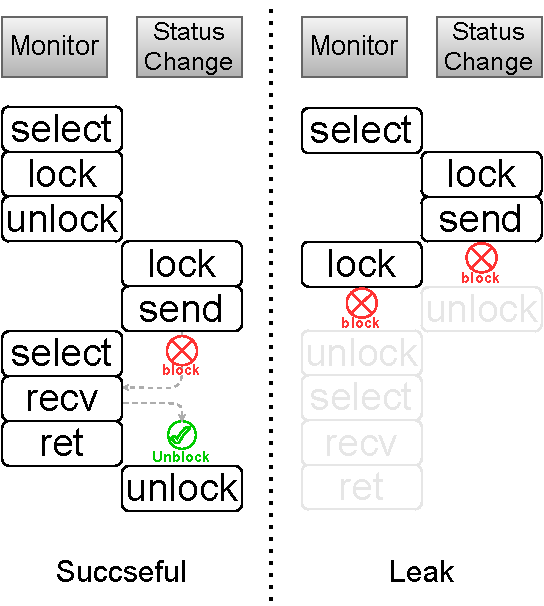
\includegraphics[width=.99\linewidth]{goat/figs/execViz_moby.pdf}
\end{minipage}
\caption{Simplified version of bug \texttt{moby28462}}
\label{listing:moby28462.minipage}
\end{listing}
